\section{Dorian Be}\label{dorian-be}

Tags: PC Alias: La scimmia alata Creatore: Davide Giocatore: Davide
Ispirazione: Harambe/Dorian Be Luogo: Kos Razza: Corvilus Classe: Monaco
Livello: 10

\section{Dorian Be}\label{dorian-be-1}

\begin{center}\rule{0.5\linewidth}{0.5pt}\end{center}

\begin{figure}
\centering
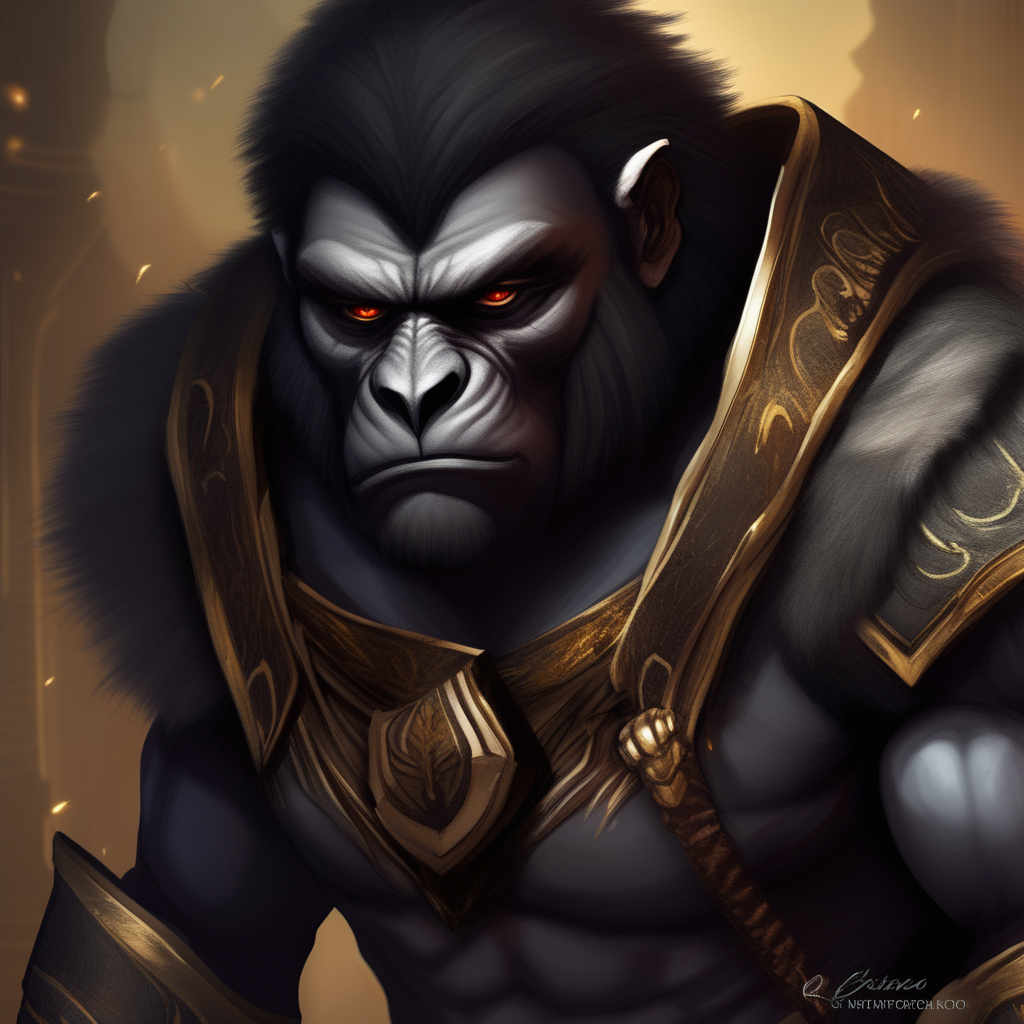
\includegraphics{create-an-image-of-dorian-be-a-heroic-character-from-a-fantasy-world-dorian-is-a-corvilus-a-race---2.png}
\caption{create-an-image-of-dorian-be-a-heroic-character-from-a-fantasy-world-dorian-is-a-corvilus-a-race---2.png}
\end{figure}

Info generali

Età: 42

Anno di nascita: 1981

Paese di nascita: XXX

Razza: Corvilus

Relazioni:

Alleati:

Nemesi:

Possedimenti importanti:

\begin{center}\rule{0.5\linewidth}{0.5pt}\end{center}

\subsection{1. Descrizione Generale}\label{descrizione-generale}

\begin{center}\rule{0.5\linewidth}{0.5pt}\end{center}

\begin{figure}
\centering
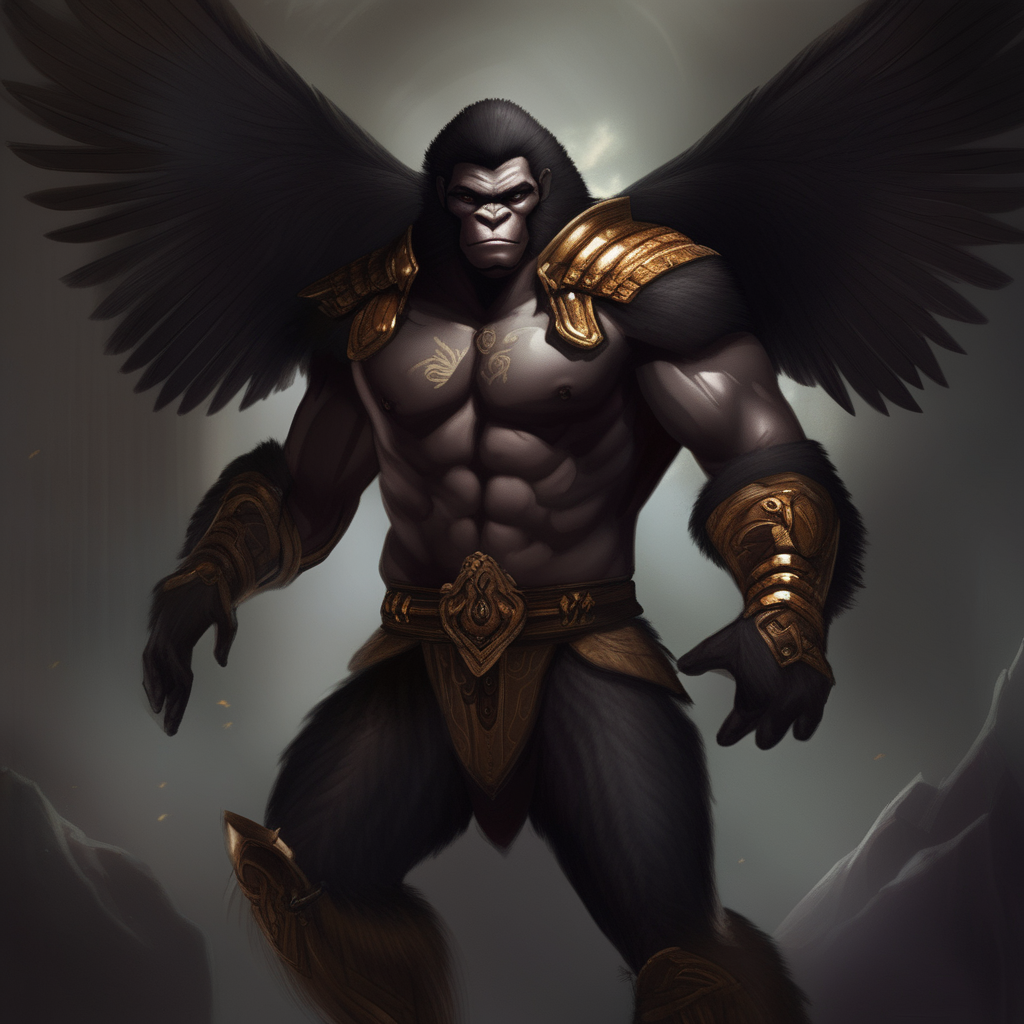
\includegraphics{create-an-image-of-dorian-be-a-heroic-character-from-a-fantasy-world-dorian-is-a-corvilus-a-race--.png}
\caption{create-an-image-of-dorian-be-a-heroic-character-from-a-fantasy-world-dorian-is-a-corvilus-a-race--.png}
\end{figure}

Dorian Be è un personaggio di spicco, noto per la sua storia di coraggio
e dedizione nel difendere coloro che sono indifesi. Appartenente alla
misteriosa razza dei Corvilus, che ricorda i gorilla alati, Dorian ha
affrontato tragici eventi che hanno cambiato il corso della sua vita.
Durante la sua carriera circense, condivisa con il suo amato fratello
Haram, ha intrattenuto le folle con spettacoli di giocoleria e abilità
acrobatiche che hanno incantato il pubblico. Tuttavia, una tragedia ha
portato alla perdita delle sue ali e alla morte di Haram, spingendo
Dorian a intraprendere un profondo viaggio di crescita personale. Rinato
come guerriero coraggioso, Dorian ha sviluppato abilità straordinarie
nel combattimento corpo a corpo e la magia arcanica. La sua personalità
compassionevole e protettiva lo ha reso un eroe errante leale, pronto ad
aiutare chiunque abbia bisogno e a portare speranza nei cuori di chi
incontra nel suo cammino.

\begin{quote}
``Tempestate di Like se vi è piaciuta la performance'' - Dorian rivolto
al pubblico
\end{quote}

\subsection{2. Biografia}\label{biografia}

\begin{center}\rule{0.5\linewidth}{0.5pt}\end{center}

Dorian Be è nato in un circo itinerante, dove insieme al suo adorato
fratello, Haram Be, intratteneva il pubblico con spettacoli di
giocoleria e abilità acrobatiche. Cresciuto in un ambiente affettuoso e
felice, la loro famiglia circense si considerava una vera e propria
famiglia allargata.

\subsubsection{\texorpdfstring{2.1 \textbf{L'Incidente
Tragico}}{2.1 L'Incidente Tragico}}\label{lincidente-tragico}

Un giorno, durante una delle loro esibizioni con bastoni infuocati, un
bambino umano si avventurò inavvertitamente nel perimetro dello
spettacolo. Il fratello di Dorian, Haram, fu distratto dal bambino e
perse il controllo dei bastoni, mettendo in pericolo la vita del
piccolo. Haram, per proteggere il bambino, si lanciò su di lui a
coprirlo, ma fu scambiato per una minaccia e ucciso da una guardia di
paese spaventata.

\subsubsection{\texorpdfstring{2.2 \textbf{La Perdita delle
Ali}}{2.2 La Perdita delle Ali}}\label{la-perdita-delle-ali}

Durante la confusione che seguì, Dorian cercò di difendere il corpo
senza vita di Haram, ma fu sopraffatto dalla folla infuriata. Durante la
lotta, subì una profonda ferita sull'ala sinistra da un oggetto
appuntito, rendendo le sue ali irrimediabilmente danneggiate. Incapace
di volare e devastato dalla perdita di suo fratello, Dorian fuggì
portando con sé il corpo del defunto Haram.

\subsubsection{\texorpdfstring{2.3 \textbf{Il Viaggio di
Crescita}}{2.3 Il Viaggio di Crescita}}\label{il-viaggio-di-crescita}

Per onorare la memoria di Haram e la loro eredità circense, Dorian
intraprese un lungo viaggio di crescita personale. Cercò maestri saggi e
guerrieri per apprendere le arti del combattimento, della magia e della
forza interiore. Durante il suo viaggio, sviluppò abilità marziali,
apprese a canalizzare l'energia arcana e mantenne vivo il legame con la
natura e le creature alate.

\subsubsection{\texorpdfstring{2.4 \textbf{La Rinascita di Dorian
Be}}{2.4 La Rinascita di Dorian Be}}\label{la-rinascita-di-dorian-be}

Dorian Be si trasformò in un combattente agile e coordinato, compensando
la mancanza delle ali con una forza fisica e spirituale incredibile.
Adottò uno stile di vita rispettoso della natura e si impegnò a
proteggere gli esseri vulnerabili, come aveva fatto con il bambino
durante l'incidente che cambiò la sua vita.

\subsubsection{\texorpdfstring{2.5 \textbf{Il Protettore dei
Deboli}}{2.5 Il Protettore dei Deboli}}\label{il-protettore-dei-deboli}

Oggi, Dorian Be è noto come un eroe errante, un guerriero
compassionevole che gira il mondo per difendere i deboli, sconfiggere il
male e mantenere vivo lo spirito del circo itinerante che un tempo
condivise con suo fratello Haram. La sua storia toccante e la sua
dedizione nell'assumere la difesa degli oppressi lo hanno reso un
personaggio famoso e rispettato in tutto il mondo di D\&D.

\subsubsection{\texorpdfstring{2.6 \textbf{Eredità di Haram
Be}}{2.6 Eredità di Haram Be}}\label{eredituxe0-di-haram-be}

Dorian Be porta sempre con sé il ricordo del fratello Haram, che
sacrificò la sua vita per proteggere un innocente. Parlando di Haram, i
suoi occhi si illuminano di amore e tristezza, mostrando il legame
indissolubile tra i due fratelli. La memoria di Haram è la forza che
guida Dorian nel suo percorso, e il nome ``Dorian Be'' è diventato un
simbolo di coraggio, protezione e speranza nel mondo di Valtara.

\subsection{3. Carriera}\label{carriera}

\begin{center}\rule{0.5\linewidth}{0.5pt}\end{center}

La vita professionale di Dorian può essere divisa in due fasi: la vita
da circense e la vita da guerriero

\subsubsection{3.1 Carriera Circense}\label{carriera-circense}

La carriera circense di Dorian Be è iniziata fin da quando era un
giovane gorilla alato. Cresciuto nel cuore di un circo itinerante, ha
imparato sin da piccolo le abilità acrobatiche, la giocoleria e il
carisma necessari per intrattenere il pubblico. Sotto la guida amorevole
dei suoi genitori adottivi e di suo fratello Haram, Dorian si è
trasformato in un abile artista circense, catturando l'attenzione delle
folle con la sua presenza carismatica e le sue abilità impressionanti.
Il duo di fratelli, Dorian e Haram, era la stella del circo, attirando
sempre il pubblico più numeroso. Le loro esibizioni erano spettacolari e
coinvolgenti, con acrobazie mozzafiato e numeri di giocoleria che
sembravano sfidare la gravità stessa. Il legame fraterno tra Dorian e
Haram era evidente sul palco, trasmettendo calore e amore agli
spettatori, che si sentivano parte di una grande famiglia circense.
L'incidente tragico che portò alla morte di Haram e alla perdita delle
ali di Dorian segnò la fine della sua carriera circense. Il circo,
devastato dalla tragedia, continuò senza di loro, ma Dorian sentì di non
poter più esibirsi senza suo fratello. Decise di intraprendere un nuovo
cammino, cercando di onorare la memoria di Haram in altri modi e di
trovare un nuovo scopo nella sua vita.

\subsubsection{3.2 Carriera da Guerriero}\label{carriera-da-guerriero}

Dopo aver vissuto un periodo di lutto e riflessione, Dorian Be iniziò il
suo viaggio di crescita personale, intraprendendo una nuova carriera
come guerriero. Sentiva di avere una responsabilità nei confronti della
sua famiglia circense e del ricordo di suo fratello. Decise che doveva
migliorarsi e diventare più forte per poter proteggere coloro che amava
e per difendere gli indifesi da eventuali pericoli. Durante il suo
viaggio, Dorian cercò insegnanti e mentori in diverse arti di
combattimento e magia. Studiò con maestri di arti marziali, imparando a
padroneggiare diverse tecniche di combattimento corpo a corpo. Inoltre,
sviluppò la sua abilità nella magia, scoprendo di poter canalizzare
l'energia arcanica e lanciare incantesimi per difendersi e aiutare gli
altri. Con determinazione e costanza, Dorian affinò le sue abilità,
combinando la forza fisica con la saggezza e la magia. Integrandole con
l'agilità acquisita nella sua carriera circense, Dorian divenne un
guerriero straordinario, capace di fronteggiare nemici e proteggere gli
innocenti. La sua connessione con la natura e le creature alate gli
conferì un legame speciale con gli animali, che spesso lo aiutano nelle
sue missioni. Ha sviluppato una particolare affinità con gli uccelli,
che considera i suoi messaggeri e compagni nell'avventura. Questo legame
speciale gli ha permesso di sviluppare uno stile di combattimento unico,
prendendo ispirazione dai movimenti aggraziati degli uccelli in volo.
Oggi, Dorian Be è un eroe errante, un combattente leale e
compassionevole, con l'abilità di proteggere gli altri con la sua forza
fisica e la magia, mentre mantiene sempre vivo lo spirito del circo
itinerante che una volta condivideva con suo fratello. La sua carriera
da guerriero è diventata una fonte di ispirazione per molti, un esempio
di come il coraggio e la dedizione possano trasformare una tragedia in
un segno di speranza e di difesa per chiunque abbia bisogno di aiuto.

\subsection{4. Personalità}\label{personalituxe0}

\begin{center}\rule{0.5\linewidth}{0.5pt}\end{center}

Dorian Be possiede una personalità profondamente empatica e
compassionevole, che è stata plasmata dalle tragedie che ha vissuto. La
perdita di suo fratello Haram ha lasciato un segno indelebile nel suo
cuore, trasformandolo in un individuo protettivo e devoto a coloro che
hanno bisogno di aiuto. È un'anima gentile, sempre pronta a tendere una
mano amica a chiunque sia in difficoltà. Nonostante la sua natura
sensibile, Dorian è anche un individuo coraggioso e tenace. Ha
affrontato numerose sfide e difficoltà nel suo viaggio di crescita,
dimostrando una determinazione inarrestabile nel superarle. La sua
dedizione nel migliorarsi costantemente, sia fisicamente che
mentalmente, lo ha reso un combattente straordinario e un alleato fidato
nei momenti di bisogno. La sua esperienza di circo gli ha donato un
senso dell'umorismo e un lato giocoso, che emergono soprattutto quando è
in compagnia di nuovi amici o quando si trova in situazioni rilassate.
Dorian è sempre pronto a intrattenere il suo gruppo con piccoli trucchi
e acrobazie, portando un po' di leggerezza e divertimento nei momenti
più cupi. Tuttavia, anche se può essere socievole e affabile, Dorian ha
anche dei momenti di intimità e riflessione. I ricordi di suo fratello
Haram possono renderlo triste o nostalgico, ma trova nella sua memoria
la forza per continuare a proteggere e difendere gli altri. La sua
connessione con la natura e le creature alate gli conferisce un profondo
rispetto per l'ambiente circostante e tutte le forme di vita. È un
ambientalista appassionato e cerca sempre di minimizzare l'impatto
negativo che può avere sull'ecosistema, prendendosi cura della fauna e
della flora che lo circondano. Dorian è anche un ascoltatore empatico,
disponibile a dare consigli o conforto quando necessario. Ha imparato
che il potere di proteggere gli altri non si limita solo alla forza
fisica, ma anche a fornire un ascolto attento e un sostegno morale.
Questo atteggiamento compassionevole gli ha guadagnato molte amicizie e
gli ha permesso di formare legami profondi con coloro che incontra nel
suo cammino.

\subsection{5. Coinvolgimenti in eventi
recenti}\label{coinvolgimenti-in-eventi-recenti}

\begin{center}\rule{0.5\linewidth}{0.5pt}\end{center}

\href{Untitled\%20Database\%20d9b94363331d4223b89fa494a1e7f74e.csv}{Untitled
Database}

\subsection{6. Scheda personaggio}\label{scheda-personaggio}

\begin{center}\rule{0.5\linewidth}{0.5pt}\end{center}

\href{Info\%20PG\%20c9e8f3e9edd64ec483415e8d3d705fc1.csv}{Info PG}

\subsubsection{Statistiche e abilità}\label{statistiche-e-abilituxe0}

\begin{center}\rule{0.5\linewidth}{0.5pt}\end{center}

\href{Abilita\%CC\%80\%207a1791510d12420c97f76cd664f79f50.csv}{Abilità}

\subsubsection{Lista magie}\label{lista-magie}

\subsection{A. Descrizione originale}\label{a.-descrizione-originale}

\begin{center}\rule{0.5\linewidth}{0.5pt}\end{center}

Dorian Be è un Corvilus (razza ispirata a dei gorilla alati) che ha
perso le sue ali durante un incidente.

Nel suo passato era un circense ambulante ed insieme a suo fratello
Haram Be viaggiavano di città in città intrattenendo le genti. Un giorno
però, durante un loro spettacolo di giocoleria in cui erano coinvolti
dei bastoni infuocati Haram venne distratto da un bambino umano che,
sfuggito dai genitori, era riuscito ad entrare nel perimetro
dell'esibizione. A causa della distrazione Haram perse il controllo dei
bastoni infuocati e, per proteggere il bambino, si precipitò su di lui a
coprirlo. Una guardia di paese si spaventò di questo gesto e sparò ad
Haram, uccidendolo.La~ folla spaventata si scatenò e Dorian, impotente e
furioso, cercò di proteggere il corpo senza vita di suo fratello. La
situazione degenerò rapidamente in una rissa violenta, poiché la folla
accusò Dorian e Haram di mettere in pericolo i cittadini con le loro
pericolose esibizioni.

Durante lo scontro, Dorian cercò di difendersi, ma fu sopraffatto dalla
superiorità numerica dei cittadini infuriati. Durante la mischia,
qualcuno prese un oggetto appuntito e gli inflisse una profonda ferita
sull'ala sinistra, causando una lesione irreparabile. Nel caos, Dorian
riuscì a fuggire, portando con sé il corpo del fratello. Si nascose per
diversi giorni, devastato dal dolore per la perdita di Haram e dalla
consapevolezza che le sue ali erano irrimediabilmente danneggiate.

Dopo essere sopravvissuto nella natura selvaggia e riflettendo sulle
tragedie che avevano colpito lui e suo fratello, Dorian decise che era
giunto il momento di onorare la memoria di Haram. Sentiva di avere una
responsabilità nei confronti della sua famiglia, di portare avanti
l'eredità del circo e di proteggere coloro che non potevano proteggersi
da soli.

Decise quindi di intraprendere un lungo viaggio per migliorarsi sia
fisicamente che mentalmente. Voleva apprendere abilità che potessero
compensare la perdita delle ali, trasformando il suo corpo e la sua
mente in un'arma difensiva potente. Si avventurò nei territori selvaggi,
cercando maestri e guerrieri saggi che potessero insegnargli le arti del
combattimento, della magia e della forza interiore.

Durante il suo viaggio, incontrò un anziano maestro di arti marziali che
lo aiutò a perfezionare il suo stile di combattimento. Scoprì anche che
poteva canalizzare l'energia arcanica attraverso le sue mani,
permettendogli di utilizzare incantesimi e magie per difendersi e
proteggere gli altri.
